\chapter{Optimized high-dimensional representation in spiking neurons}
The implementation of a Semantic Pointer Architecture in a spiking neural network requires the representation of high-dimensional vectors.
While the standard NEF already provides us with a method to do this, it does not tell us the best way to do so.
A good representation will try to minimize the error or noise in the representation.
Alternatively, if the error is sufficiently small, it allows to reduce the number of neurons which reduces the simulation run time.
I previously proposed an optimization method for the representation~\parencite{gosmann216}, which improved the accuracy of SPA operations by up to 25 times.
Here, I will describe a more general applicable method that matches or exceeds the performance of the method among some other advantages.

\section{Types of error in neural representations}
In the NEF the total representational error is given by
\begin{equation}
    \errtotal^2 = \left\langle \errtotal^2(\vc x) \right\rangle_{\!\vc x \in \repspace} = \left\langle \norm{\vc x - \hat{\vc x}(t)}^2 \right\rangle_{\!t,\,\vc x \in \repspace} \text{.}
\end{equation}
As detailed by \textcite[47--48]{eliasmith2003} the total error is constituted out of the error caused by spiking noise $\errnoise$ and the error due to the static distortion $\errdist$ from the non-perfect decoding:
\begin{align}
    \errtotal^2(\vc x) &= \errnoise^2(\vc x) + \errdist^2(\vc x) \\
    \errnoise(\vc x) &= \left\langle \norm{\hat{\vc x}(t) - \langle \hat{\vc x}(t) \rangle_{\!t}}^2 \right\rangle_{\!t} \\
    \errdist(\vc x) &= \norm{\vc x - \langle \hat{\vc x}(t) \rangle_{\!t}}^2 \text{.}
\end{align}
The relation of the error terms is explained by the partitioning of the sum of squares in ordinary least squares model (which is used to solve for decoders in the NEF).
Note that the noise error will depend on the decoding synapse.
As $\syntau \rightarrow \infty$, the noise error will approach zero ($\errnoise \rightarrow 0$).
Because the synapse limits how fast the neural representation can be updated, we get a trade-off of the noise in the system and how fast it reacts to new inputs.

Due to the neuron nonlinearities finding analytical solutions for the error terms is likely not possible (except for constrained special cases).
However, we can estimate the error terms from computational experiments.
To do so, we sample $\vc x \in \repspace$ or use a regular grid of $\vc x$.
Each $\vc x$ is then presented for some duration $\Delta t_{\ped{ss}}$ to reach the steady state and then $\hat{\vc x}(t)$ is measured for some sample duration $\Delta t_{\ped{sample}}$.
Appropriate durations will depend on the decoding synapse (longer synapses require more time to reach the steady state) and firing rate (a longer sampling duration is required for accurate estimates with low firing rates).

As the dimensionality of the higher-dimensional space increases, it becomes increasingly difficult to cover the whole space with samples from $\repspace$.
Most of the time, though, we can treat the space as an isotropic hyper-ball, i.e.\ it does not matter along which direction we move through the space.
This requires that the NEF ensemble's encoders are uniformly sampled from the hyper-sphere surface which is usually the case (but there are some exceptions like certain implementations of a product network,~\cite{gosmann2015-1}, or thresholding ensembles, \cref{sec:thresholding}).
Without loss of generality, we assume the representational radius of the hyper-ball to be $r = 1$ (as it is purely a scaling factor).
The isotropy property allows us to cut through the center of the hyper-ball with a one-dimensional line.
Measuring the error $\err(x) = \err(\vc x)$ at $m$ regular spaced points $\vc x_i = (x_i, 0, \dotsc, 0)\Tr$ with $x_i = i * \Delta x - \Delta x/2,\ \Delta x = 1/m,\ 1 \leq i \leq m$ along such a line, the mean error for the hyper-ball can be estimated as
\begin{align}
    \err &= \frac{\sa_{\dims}}{\ballvol_{\dims}} \sum_{i=1}^{m} \err(x_i) \cdot \Delta x \cdot r(x_i) \\
    \sa_{\dims} &= \frac{2 \pi^{\dims/2}}{\gammafn(\dims/2)} \\
    \ballvol_{\dims} &= \frac{\pi^{\dims/2}}{\gammafn\!\del{\frac{\dims}{2} + 1}} \\
    r(x) &= \frac{1}{q} \sum_{i=1}^{q} \abs{x - \del{1 + \frac{1}{q}} \frac{\Delta x}{2} + i \frac{\Delta x}{q}}^{\dims - 1}
\end{align}
where $\sa_{\dims}$ is the $\dims$-dimensional solid angle, $\ballvol_{\dims}$ the volume of a $\dims$-ball with radius $\radius = 1$, and $r(x)$ estimates the radius to the power of $\dims-1$ for an $x$ with $q$ evaluation points.
This later estimation of the radius across the $\Delta x$ interval is necessary to not under- or overestimate the integral by a large amount.
This were to happen if only the radius at the exact evaluation point would be used.


\section{Properties of the error in neural representations}
When looking at the representation of a spiking neural network, the noise error is the main factor to consider.
It will go down by $\bO(1/\sqrt{n})$ where $n$ is the number of neurons (\cref{fig:noise-error}a), whereas the distortion error will decrease by $\bO(1/n)$ and is thus dominated by the noise error~\parencite[Fig.~2.6]{eliasmith2003}.
In contrast, for rate neurons $\errnoise = 0$ and only the distortion error is relevant.
Furthermore, with the Nengo defaults the noise error in the NEF the increase in the noise error with dimensions $\dims$ will be in $\bO(d)$ (\cref{fig:noise-error}b).
\begin{figure}
    \centering
    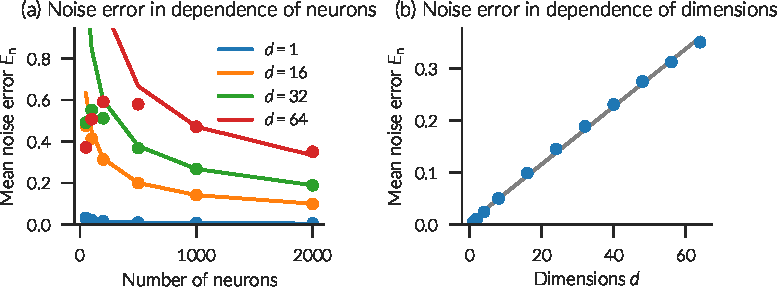
\includegraphics{figures/noise-error}
    \caption{The mean noise error $\errnoise$ in dependence of (a) the number of neurons and (b) the number of dimensions. Scatter points show empirically determined values with 95\% confidence intervals smaller the marker size. Solid lines in (a) are extrapolated from the mean values for \num{1000} neurons assuming the noise error is in $\bO(n)$. The solid gray line in (b) is a linear regression through all show data points.}\label{fig:noise-error}
\end{figure}

When looking at the error along a line through the hyper-ball (\cref{fig:error-linecut}), it becomes apparent that the distortion is mostly flat, but increases near the surface.
This becomes more pronounced as the dimensionality increases.
The noise error will be slightly larger in the center of the ball than towards the surface with higher dimensionalities (it is a flat line for $\dims = 1$).
This is caused by the uniform sampling of evaluation points from the hyper-ball (\cref{fig:circle-covering}).
When looking at the convex hull of the sample points, this hull will always be smaller than the hyper-ball (even if some evaluation points are exactly on the surface).
Thus, parts of the hyper-ball near the surface are not covered by the evaluation points and will not be considered in the least squares optimization of the decoders.
As the number of dimensions increases, this will become a bigger problem as the volume for a hyper-ball goes to zero as $\dims \rightarrow \infty$ (all of the ball will be surface).
To show that this distortion is indeed caused by the partial covering, we can increase the radius of the hyper-ball for sampling the evaluation points slightly to cover more of the unit-ball (\cref{fig:error-radius-scale}).
While this makes the distortion more even (mean distortion reduced by \num{0.011}), it unfortunately also increases noise level (by \num{0.019}) distortion because evaluation points now have a larger spacing.
These and future values in this chapter are statistically significant with $p \approx 0$ as long as not otherwise noted.
The $p$-value has been determined with bootstrapping.
\begin{figure}
    \centering
    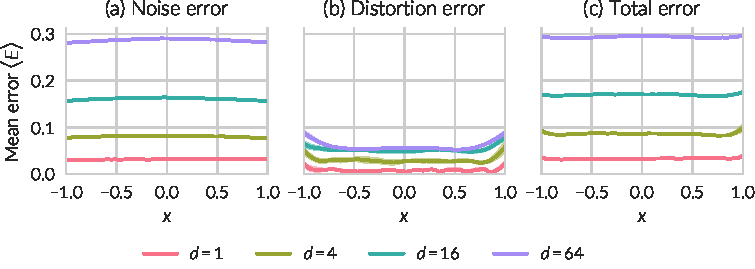
\includegraphics{figures/error-linecut}
    \caption{Mean error along a line cut through the $d$-dimensional hyper-ball with $50\dims$ neurons. The (a) noise error component, (b) distortion error component, and (c) the total error are shown. The shaded regions indicate 95\% confidence intervals.}\label{fig:error-linecut}
\end{figure}
\begin{figure}
    \centering
    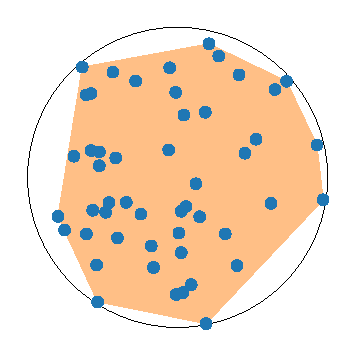
\includegraphics{figures/circle-covering}
    \caption{Covering of the two-dimensional unit-circle with 50~uniformly sampled evaluation points. The orange, shaded region shows the convex hull which fails to cover the area close to the circle boundary.}\label{fig:circle-covering}
\end{figure}
\begin{figure}
    \centering
    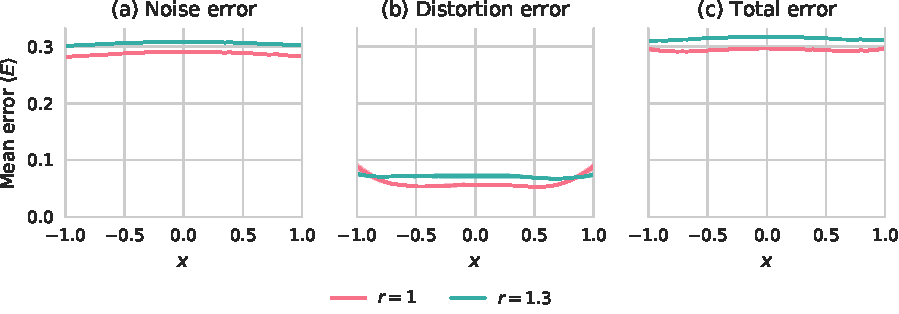
\includegraphics{figures/error-radius-scale}
    \caption{Mean error along a line cut through the \num{64}-dimensional hyper-ball with \num{3200} neurons and different radii $r$ from which evaluation points are picked. The shaded regions indicate 95\% confidence intervals.}\label{fig:error-radius-scale}
\end{figure}

Vectors in the SPA are often of unit-length and thus a good, low-distortion representation of the hyper-ball surface is desirable.
Unfortunately, I am not aware of any method to improve the current state.
To completely cover the ball in a convex hull of evaluation points, it is necessary to place some evaluation points outside of the ball which will cover space and optimize for space outside of the representational space.
This will lead to a trade-off of flatness of the distortion and baseline of the distortion.


\section{Effect of the intercept distribution on noise and distortion}
The intercepts in Nengo are chosen to be uniformly distributed by default.
In higher dimensions, this has the effect that most neurons are either almost never or almost always active for values in the representational space (\cref{fig:act-proportion}).
These neurons contribute only minimally to the representation as a neuron that is always in-active does not provide any information about the actually represented value.
But also always active neurons only contribute minimally to the representation.
Here the firing rate will still vary a bit about the representational space, but for typical neuron models the response curve is steepest closest to the intercept.
That mapping of a small change in the represented value to a large change in firing rate allows for a less noisy decoding as a single spike will change the decoded value less.
\begin{figure}
    \centering
    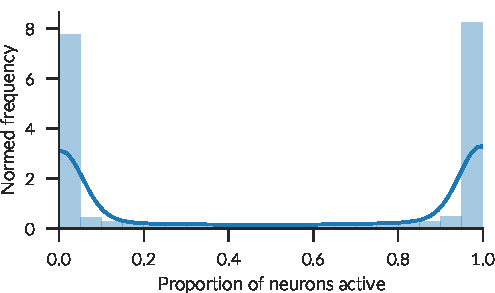
\includegraphics{figures/act-proportion}
    \caption{Histogram (shaded bar plot) and kernel-density estimate (line) of the proportion of neurons active for uniformly sampled 64-dimensional vectors.}\label{fig:act-proportion}
\end{figure}

Thus, a better intercept distribution should have less neurons that are barely ever active, but should also distribute the intercepts so that there is an even distribution of the fraction of space a neuron is active for.
The latter criterion can be achieved by distributing the intercepts according to $\csdist(\dims+2)$ where $\csdist(d_{\csdist})$ is the distribution of cosine similarities between random uniformly distributed $d_{\csdist}$-dimensional unit-vectors.
Its probability density function is given by (\cref{fig:cosine-sim}, derivation in \cref{apdx:cosine-sim})
\begin{equation}
\pcs(x; d_{\csdist}) = \frac{1}{B\!\del{\frac{1}{2}, \frac{d_{\csdist} - 1}{2}}} \cdot \del{1 - x^2}^{\del{d_{\csdist} - 3} / 2},\quad x \in [-1, 1] \text{.}\label{eqn:pcs}
\end{equation}
$\csdist(\dims+2)$ is equivalent to the distribution of single coordinates of points uniformly sampled from the $\dims$-dimensional unit ball~\parencite{voelker2017}.
Thus, by using this intercept distribution, the frequency of intercepts corresponds to the distribution $\langle \vc x, \enc \rangle,\ \vc x \in \repspace$, i.e.\ the projection of values in the representational space projected onto the (uniformly distributed) neuron encoders.
\begin{figure}
    \centering
    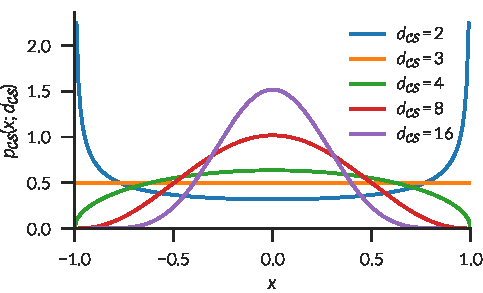
\includegraphics{figures/cosine-sim}
    \caption{PDF $\pcs(x; d_{\csdist})$ of the cosine similarity distribution.}\label{fig:cosine-sim}
\end{figure}

\Cref{fig:act-cs} shows compares the relative amount of neurons that do not fire for any of the evaluation points.
For the standard uniform distribution, this fraction rises to above \num{0.35}, but is close to zero with the cosine similarity intercept distribution.
When we look at the actual error (\cref{fig:error-cs-intercepts}), we see that it is reduced (\num{-0.130}).
This is mainly due to a reduction in the noise error.
The distortion seemingly increases, but because most of the volume of the space is near the surface and the distortion there ends up a little bit lower, the total distortion will also decrease (\num{-0.020}).
However, where the space is distorted changes.
While the uniform distribution leads to an even distortion except towards the hyper-sphere surface, the cosine similarity distribution gives a distortion that varies more across the space.
In particular, there is a ring of higher distortion between the center and the surface of the hyper-ball and another such ring around the surface.
\begin{figure}
    \centering
    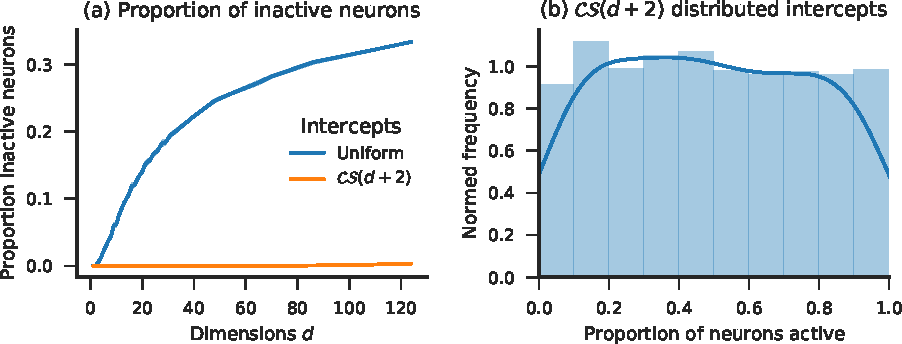
\includegraphics{figures/act-cs}
    \caption{(a) Proportion of neurons inactive for all \num{10000} uniformly sampled $\dims$-dimensional vectors. The proportion is plotted for neural ensembles with a uniform intercept distribution (blue) and intercepts distributed according to $\csdist(\dims + 2)$ (orange). The shaded areas denote 95\% confidence intervals. (b) Histogram (shaded bar plot) and kernel-density estimate (line) of the proportion of neurons active for uniformly sampled 64-dimensional vectors when distributing intercepts according to $\csdist(\dims + 2)$.}\label{fig:act-cs}
\end{figure}
\begin{figure}
    \centering
    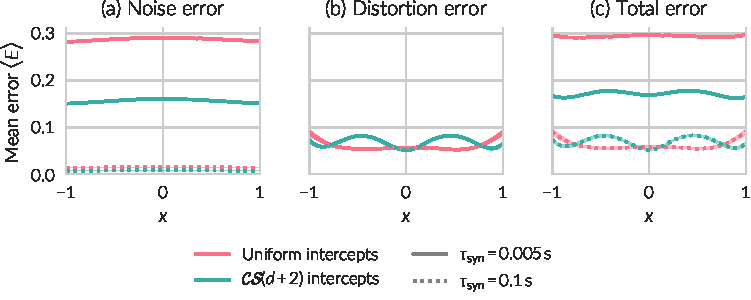
\includegraphics{figures/error-cs-intercepts}
    \caption{Mean error along a line cut through the 64-dimensional hyper-ball with 3200 neurons and different intercept distributions. The shaded regions indicate 95\% confidence intervals.}\label{fig:error-cs-intercepts}
\end{figure}

In general, there will be a noise-distortion trade-off.
Reducing the noise error by changing the intercept distribution, will lead to a more uneven distortion and can potentially increase the total distortion.
For spiking neurons with short synaptic time constants, the noise error is usually much higher and thus the change in the distortion will often be negligible.
Longer synaptic time constants will shift this trade-off as the noise error will be lower.
Still, for biological realistic time constants of up to \SI{0.1}{\second}, the cosine similarity intercept distribution will perform better (by \num{0.021}).
It is also worth noting that this trade-off will be slightly affected by the regularization term when solving for the decoders.
A will decrease the noise as the decoders get less sensitive to small fluctuations, but increases the distortion towards the hyper-sphere surface.
The opposite effects are observed with less regularization.

Interestingly, the cosine intercept distribution does not only reduce the noise by a constant factor compared to the uniform distribution.
Rather it improves the scaling of the noise error from $\bO(d/\sqrt{n})$ to $\bO(d^{3/4}/\sqrt{n})$ (TODO figure).

So far we only considered spiking neurons, but the NEF also allows the usage of rate neuron models.
In that case, the noise error will be zero because the firing rate can be represented with arbitrary precision.
With the default parameters, the cosine similarity distribution still gives a slightly lower total distortion (TODO figure).
However, due to the non-existent noise, the default regularization of $\gamma = 0.1$ too large and a lower error can be obtained by reducing the regularization to $\gamma = 0.01$.
Then the uniform distribution will perform better (TODO figure), while the cosine similarity intercept distribution increases the distortion.

Here I focused on the cosine similarity intercept distribution because it works well over a wide range of neuron types and parameters as well as reducing to the uniform distribution when $\dims = 1$.
Despite that, other intercept distributions can be used and might produce even better results for a fixed set of parameters (or for the approximation of a specific non-linear function).
TODO takes a more exhaustive look at different choices and compares them.

It is also worth to note that the present analysis assumes that all values in the representational space $\repspace$ are uniformly distributed.
If certain values appear more frequently than others, the optimal intercept distribution might change.
The experimental procedure used here to compare intercept distributions might still be used, but the error needs to be weighted by the frequency of the represented values $\vc x$.


\section{Optimized Semantic Pointer Representation and Manipulation}
The NEF only requires multiple vector dimensions to be represented in a single ensemble if functions with a nonlinear interaction of the individual dimensions is decoded.
Such interactions are rarely needed in the Semantic Pointer Architecture and there is a number of reasons to split up the $\dims$-dimensional vector into $q$ vectors of $\dims_q = \dims / q$ dimensions.

First of all, solving for decoders requires the inversion of an $n \times n$ matrix with a runtime complexity of $\bO(n^3)$ where $n$ is the total number of neurons in the ensemble.
When instead using $q$ ensembles with $n/q$ neurons each to represent $\dims_q$ segments of the vector, only $q$ inversions of $n/q \times n/q$ matrices are required, which give a runtime complexity of only $\bO(n^3/s^2)$.
Thus, solving for the decoders can be a lot more efficient when splitting up a vector into multiple ensembles for the representation.

Second, the noise error grows only in $\bO(\sqrt{q/n})$ if $\dims_q$ is kept constant.
In other words, adding $\dims_q$ more dimensions, requires only $n/q$ additional neurons to keep the noise error constant.

Splitting up the input space in this manner, however, introduces a slight complication.
While we can assume the full vectors $\vc x \in \repspace$ to be uniformly distributed, this is not the case for the $\dims_q$-dimensional subvectors.
The distribution of the subvectors will cluster around shorter vectors.
One way to account for that, is to reduce the representational radius $\radius$ of the ensembles which will improve the representation of the most common vectors, but worsen the representation of subvectors that fall outside of that radius (which might still occurs occasionally).
\Textcite{gosmann216} describes in detail how to find a good value for $\radius$.

Here, I use a different method, where both the intercept distribution and evaluation point distribution are set to the cosine similarity distribution $\csdist(\dims + 2)$ (note that this uses the dimensionality of the complete vector, not $\dims_q$).
In addition to before, the distribution of evaluation points accounts for the fact that the represented values are no longer uniformly distributed.

To verify the performance, I repeated the benchmarks from \textcite{gosmann216}\@.
A randomly moving unit-length semantic pointer is fed as input to the set of ensembles and the distribution of resulting error in the representation is measured (TODO fig).
The new method of setting the intercept and evaluation point distributions performs almost as well as the previous radius adjustment method for $q = \dims$ and better if $q < \dims$.
It thus generalizes to a wider range of cases.
Instead of adjusting the hard radius cutoff, the distributions result in the representational quality slowly fading out proportional to the frequency of values in that range.

Besides the representation of a vector, the choice of intercept and evaluation point distribution improves the accuracy of the dot product to the level of the radius adjustment method (TODO figure) and surpasses it for the circular convolution operation (TODO figure).
